\documentclass[11pt,a4paper,openany]{book}

% \usepackage[german]{babel}	%in case you want to write a german thesis

%settings for generation of titlepage, index and table of content
\include{sections/Settings}

%definitions for easier costumization
\def \subtitle {Robot Extensible Communication Toolkit}
\def \year {2023/24}
\def \authors { \parseauthor{Projectmanagement. Rust TCP/UDP and BLE Interface}{Jeremy Sztavinovszki}{5CHIF}\\
	\parseauthor{Rust gRPC Interface and interacting with in memory sqlite databases}{Christoph Fellner}{5BHIF} \\
	\parseauthor{C++ gRPC interface and library for communication}{Maximilian Dragosits}{5CHIF} \\
	\parseauthor{RECT Tool and Python gRPC interface and library for communication}{Timon Koch}{5CHIF} }
\def \supervisor { Harald R. Haberstroh }
\def \declauthors{ 	Jeremy Sztavinovszki & Christoph Fellner \\
	Timon Koch & Maximilian Dragosits}
% \def \declauthors{ Vor- und NACHNAME & Vor- und NACHNAME \\ Vor- und NACHNAME}	% for three authors

\addbibresource{main.bib}

\begin{document}
	%include titlepage
	\input{sections/titlepage}
	
	%include acknowledgements, abstract and documentation
	
	\pagestyle{plain}
	
	\frontmatter
	
	\pagenumbering{roman}
	\input{sections/declarationof}
	
	\tableofcontents
	
	\chapter{Acknowledgement}

The authors would like to thank their respective families, the HTBLuVA and robo4you 
for their support throughout the process of creating this diploma thesis. 

	

\chapter{Kurzfassung}

\textbf{Author: Sztavinovszki}

\vspace{10mm}

Eine der am meisten in der Robotik verwendeten Software Suiten ist das sogenannte Robot Operating System \footcite{ros-site} (kurz ROS).
Es ist eine Sammlung von Werkzeugen und Packeten, die verwendet werden, um hoch performante Robotik Systeme zu entwickeln und es abstrahiert
die Kommunikation zu Topics und Messages, die man in ROS-Bag Files aufzeichnen und abspielen kann. Das erlaubt es entwicklern sich auf die tatsächlichen Probleme der Entwicklung zu konzentrieren und sich nicht darum kümmern zu müssen Kommunikation neu zu implementieren.
ROS erlaubt außerdem die simulation Zahlreicher Komponenten von Robotern, welche man meistens als Digitale Zwillinge bezeichnet.
Einer der größten Nachteile, die ROS mit sich bringt ist die Komplexität und der Eigensinn, bei der Entwicklung. Diese Komplexität führt außerdem zu Performance einbußen, welche vor allem die Verwendbarkeit auf weniger Leistungsstarken Geräten, wie zum Beispiel dem KIPR Wombat Controller \footcite{wombat-controller}, welcher bei Schülern wegen seiner Kostengünstigkeit und Verwendbarkeit zum Einsatz kommt.

\medskip

Diese Arbeit wird erkunden, wie man eine Software ähnlich zu ROS implementiert. Es werden Probleme, wie zum Beispiel Inter Prozess Kommunikation \footcite{ipc-begriff}, Kommunikation durch Bluetooth Low Energy (BLE), TCP und UDP, und die Implementation von Kommunikations Libraries für verschiedene Programmiersprachen


\chapter{Abstract}

\textbf{Author: Sztavinovszki}

\vspace{10mm}


% Context or background information; general topic; specific topic.
In robotics one of the most important topics over the last couple of years has been communication. Communication doesn't only concern a robot being remote controllable. Mimimi keine Ahnung. 

% central questions or problem statement

% what's already known, what previous research has shown

% main reasons, rationale, goal for research

% research and or analytical methods

% main findings, results or arguments

% significance or implications


	
	%include thesis
	
	\mainmatter
	\pagenumbering{arabic}
	
	\chapter{Introduction}


\vspace{2mm}

\section{Motivation}
\textbf{Author: Sztavinovszki}
In almost every robotics application nowadays you need some kind of communication. Wether it is a robot communicating
its data to a home-base, or two robots sharing data with one another. Over the past years communication has drastically
improved with new protocols and technology, such as Bluetooth Low energy.

\section{Goal}
\textbf{Author: Sztavinovszki}

\section{History}

\section{Project Management}
\textbf{Author: Sztavinovszki}

\section{Outline}
%\section{Section}
%More text. \lipsum[1] See Figure~\ref{pic:example}.

%\begin{figure}[h]
%	\centering
%	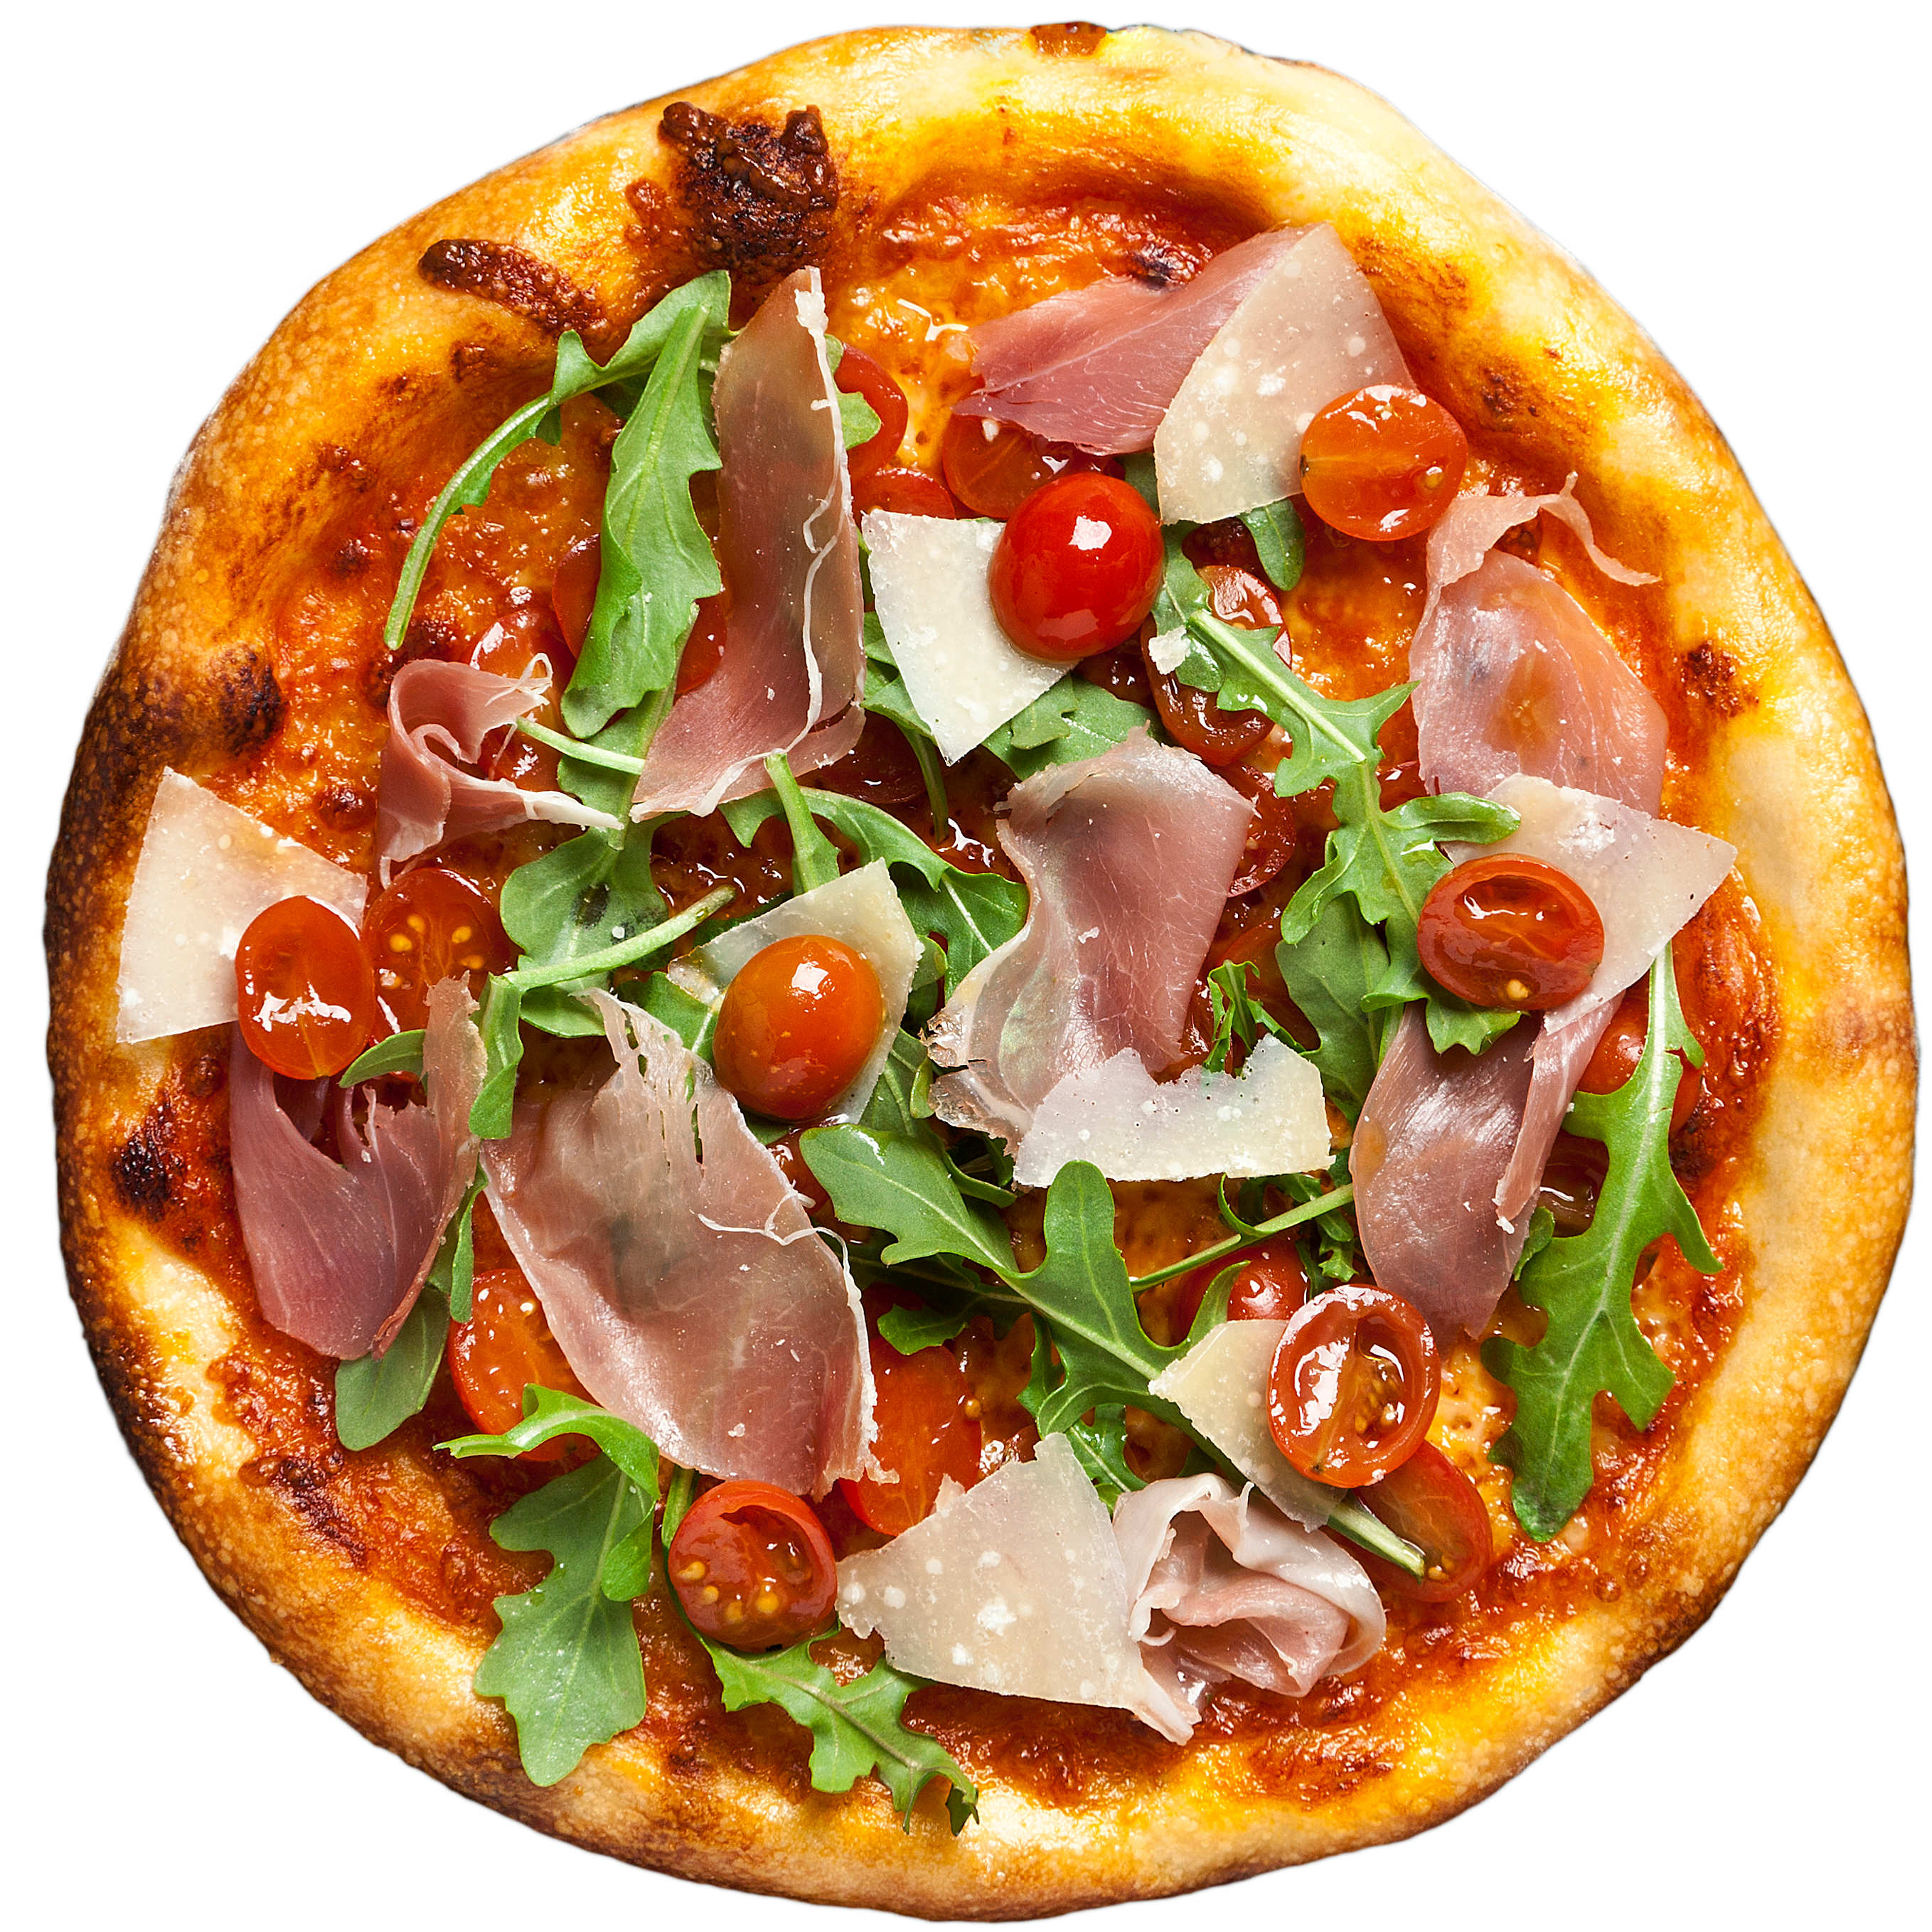
\includegraphics[width=2.5in]{img/example.png}
%	\caption{Picture description.}
%	\label{pic:example}
%\end{figure}

%\subsection{Subsection}
%\lipsum[1]

%\subsection{Subsection}
%\lipsum[1] See Table~\ref{tab:example}.

%\begin{center}
%	\begin{tabular}{| l | l | l |}
%		\hline
%		\bfseries Header 1 & \bfseries Header 2 & \bfseries Header 2 \\
%		\hline
%		Text & text & text \\
%		\hline
%		Text & text & text  \\
%		\hline
%		Text & text & text  \\
%		\hline
%	\end{tabular}
%	\label{tab:example}
%\end{center}

%\lipsum[1] Some references can be found at \footcite{robo4you} or at \footcite{Hope_Learning_TensorFlow}.
%

\filbreak

	%\chapter{Study of Literature Sztavinovszki}

\textbf{Author: Jeremy Sztavinovszki} 

\section{The Rust Book}
% summary and main takeaway


\section{Network Programming with Rust}
% summary and main takeaway



\section{Main Takeaways}

\section{Getting Started with Bluetooth Low Energy}
Getting Started with Bluetooth Low Energy\footcite{ble_book} is a book giving deep insight into
the inner workings of Bluetooth Low Energy. The first four chapters are especially useful to this
work and are summed up in the following sections.

\subsection{Chapter 1. Introduction}
The introduction explains the history of Bluetooth Low
Energy from its start as Wibree, over the adoption by the Bluetooth Special Interest Group, to
the status at the time of the writing of the book. The chapter then goes on to explain the difference
to Bluetooth Classic. Key Limitations like Data througput and Operation range as well as possible network
topologies and the difference of Protocols versus profiles are also explained.  

\subsection{Chapter 2. Protocol Basics}
The second chapter goes over the different layers and protocols of Bluetooth Low Energy explaining the importance
and use for each of the layers and also covering the Generic Attribute Profile and the Generic Access Profile. It
provides explanations for the frequency hopping and modulation done in the physical layer and many other specifics
in the other layers.

\subsection{Chapter 3. GAP(Advertising and Connections)}
The third chapter explains concepts like roles, such as Broadcaster and Observer, and explains how each of them work.
It gives explanations of the modules and procedures included in the General Access Profile. After that section the Security
Manager and General Security constructs, such as Address Types, Authentication and Security Modes are covered. Lastly the GAP
service and the format in which data is sent over advertisements is covered.

\subsection{Chapter 4. GATT(Services and Characteristics)}
This chapter goes on to explain the roles defined in the Generall Attribute Profile and covers UUIDs.
Then the most important concept, Attributes, are explained. This chapter along with the documentation for the library this work uses for BLE solidified, that L2CAP is more suitable for this work. 
% Bla bla bla. Hier weiter schreiben.

\subsection{The Remaining Chapters}
The remaining covers go over specific hardware platforms, debugging tools, application design tools and platform specific mobile
programming and were not as important as the previous four chapters. Therefore they are not covered here.

\subsection{Main Takeaways}
The book provides great explanations of many difficult topics through text as well as visual aids. The main takeaways for this work are, that L2CAP is better suited for its purposes and better general knowledge of the BLE and its stack.


\filbreak

	%\input{sections/methodology}
	\chapter{Technology}


\section{Wombat}

\section{Python}

\section{C++}

\section{Rust}
\textbf{Author: Jeremy Sztavinovszki}

Rust is a general purpose multi paradigm programming language used in many fields ranging from embedded programming to web development. Although it is a relatively young language, having released its version 1.0 on May 15th 2015, it has seen great adoption from developers and has a big community. The language tries to be as fast as possibly, while still remaining memory-safe, which it achieves using its borrow checker. Even though it is possible to write unsafe code in Rust, that is not checked by the borrow checker, it is custom to keep the unsafe parts as small as possible.
Rust has a great ecosystem driven by the Rust Foundation and the Rust community. There are many tools, such as cargo, or rust-gdb, that provide great developer experience.
Right now there is now standardized async-runtime, so you normally use runtimes like tokio, async-std, or smol for programming asynchronously.

\section{gRPC}

\section{Bluetooth Low Energy}
\textbf{Author: Jeremy Sztavinovszki}

Bluetooth Low Energy (BLE) is a low powered, low cost, low bandwidth radio communication technology, that was originally developed at Nokia in a project named Wibree. It was later noticed by the Bluetooth Special interest group and became part of the Bluetooth 4.0 Core Specification. Nowadays it is often used in all things ranging from wireless headphones to IOT devices and has seen great adoption in many different areas. The BLE protocol Stack, like others (e.g. TCP/IP) is separated into different layers. The layers are split into 3 overarching layers. which are the Application, Host and Controller layers.

\subsection{Application-Layer}
Much like the TCP/IP-Stack the BLE-Stack also comes with an Application-Layer. The Application-Layer is the highest layer in the stack and is responsible for containing logic, user interface and handling the data of the application using BLE. It often determines which usage model is used in the Host-Layers.
It is the layer that bundles all of the functionality of BLE together and abstracts it in such a way, that it is useable for ordinary users.

\subsection{Host-Layer}
The Host-Layer itself splits off into several layers. It is made up of all layers above the Host Side HCI, except the Application Layer, but not only that. It also contains profiles, which
determine how the protocols in the host layer should work with oneanother depending on the usage model, that has been chosen by the Application.

\subsubsection{Generic Access Profile GAP}
The Generic Access Profile, or GAP defines which role a BLE-Device has in communication. These roles determine how the device, as well as other devices act, when sending or receiving data.
A BLE device can take on 4 distinct roles, which are as follows.

\begin{itemize}
\item{Broadcaster}
\item{Observer}
\item{Peripheral}
\item{Central}
\end{itemize}


\subsubsection{Generic Attribute Profile GATT}
GATT

\subsubsection{Logical Link Protocol and Adaptation Protocol L2CAP}
L2CAP

\subsubsection{Attribute Protocol ATT}
ATT

\subsubsection{Security Manager Protocol SMP}
test

\subsubsection{Host Controller Interface HCI (Host side)}
test

\subsection{Controller}
The controller is the layer works closely with the hardware. It contains the following layers

\subsubsection{Host Controller Interface (Controller side)}
test

\subsubsection{Link Layer LL}
Hidden behind the HCI is the Link Layer. It is usually implemented as a conglomeration of custom hardware, as well as software it is the only part
of the protocol stack, that needs to have real-time capabilities, because it needs to work with the timing requirements defined by the specification.
In order to avoid overloading the CPU running the software layers of the stack, the easily automated, or computationally expensive parts are implemented in circuitry.


\subsubsection{Physical Layer PHY}
The physical layer is made up of the actual hardware, that is capable of modulating and demodulating the analog signals sent by radio and turning them into digital information. It uses the 2.4GHz ISM \footcite{ism} radio band, which it splits into 40 channels (37 for transmitting data and 3 for advertising connections and broadcasts) from 2.4GHz to 2.4835GHz. It uses FHSS to avoid radio interference, which is important, because classic bluetooth, as well as 2.4GHz use the same frequency band. The modulation rate chosen for BLE is 1.0Mbit/s, which means that is the physical throughput limit. However because of protocol overhead this physical throughput level is never reached.

\section{Libraries}

\subsection{Rusqlite}
\textbf{Author: Christoph Fellner}

Rusqlite is an ergonomic wrapper for using SQLite from Rust similar to rust-postgres. It provides an easy-to-use interface to work with SQLite databases. Using the functions provided by rusqlite you can perform all the common database operations, such as creating tables, inserting Data, querying data, and more simply within your code. 
We choose this library for SQLite mainly because of three reasons:
\begin{enumerate}
    \item \textbf{Portability:} SQLite databases can be used across different platforms and operating systems. Given the fact that RECT operates on different small Controllers, portability is very important.
    \item \textbf{Configuration:} There is no need for any complex setup or configuration when working with SQLite. We only need a few tables to work with, so having to configure a database on each controller wouldn't be worth the effort.
    \item \textbf{Local:} SQLite doesn't need any separate server or installation. It contains all the features we need in a small an independent package.
\end{enumerate}

In our case we use rusqlite in order to save the config.json file, containing date for the available connections. Accessing the Data from the database is simply much quicker and saver than reading from the file when we need it. 

\subsection{Serde}
\textbf{Author: Christoph Fellner}

Serde is a framework for rust, used for \textbf{ser}ializing and \textbf{de}serializing data structures efficiently and generically. You can find a detailed serde overview \href{https://serde.rs/}{here}.

Serde provides functions to deserialize JSON-files in a simple and quick way, this allows us to use the data from the config.json file in our program with just a few lines of code.

With serde we deserialize the data from the JSON-file into a self-made rust structure, which allows us to use the data properly.  

\subsection{Tokio}
\textbf{Author: Christoph Fellner}

Tokio is asynchronous runtime for rust. In rust asynchronous code doesn't run on it's own in order to make it work the programmer has to use a runtime like Tokio. You can find more in depth descripton of Tokio \href{https://tokio.rs/tokio/tutorial}{here}. 

We picked Tokio because it is the most widely used runtime for async rust code. There are also a lot of Tutorials for Tokio and it is fairly simple to use.

Tokio as our asynchronous runtime allows us to execute multi-threaded async code safely.  

\subsection{Tonic}
\textbf{Author: Christoph Fellner}

Tonic is a rust framework that implements gRPC.

\filbreak

	\chapter{Implementation}

\section{CommLib}
\textbf{Author: Jeremy Sztavinovszki} 
The Communication Library, or CommLib for short is the part of the RECT stack, that handles all of the communication between the hosts over traditional protocols, like TCP, UDP and BLE.
This requires it to be especially performant. In order to avoid premature optimization however, the first part of this section on the implementation of the CommLib will only cover the first versions
of the code written to get the Library to work. After the first implementation there will be benchmarks and some profiling, in order to get a grasp on which aspects of the library need to be
optimized. The second section will then cover how these results were incorperated into designing a more polished version of the CommLib.

\subsection{Setting up the Library} 
The first steps of setting up the library are more or less the same as in any other rust project. First the project is initialized with \verb+cargo new --lib <rust-name>+. This creates a
new folder with the name specified in \verb+<library-name>+ and generates some files like Cargo.toml and src/main.rs. After this step is done the needed libraries for RECT are added to the
project through \verb+cargo add <dependency-name> -F <dependency-name>/<feature-name>+ these dependencies are the pulled and built by cargo (Rust's build tool) upon the initial build of the
project. The first iteration of the project then had the following dependencies:

\begin{itemize}
	\item{tokio}
	\item{bluer}
	\item{anyhow}
\end{itemize}

All in all the commands used to generate the CommLib project and install all dependencies looked like this:
\newline
\begin{minipage}{\textwidth}
	\begin{lstlisting}[language=bash, caption=Setup Commands for CommLib]
		cargo new --lib comm_lib && cd comm_lib
		cargo add tokio bluer anyhow -F tokio/full,bluer/full
		cargo build
	\end{lstlisting}
\end{minipage}

\subsection{First Implementation}
The first part of the implementation that was tackled was to create an abstraction layer over the existing protocols that RECT uses.
in order to have a nice and clean interface to work with and to avoid having to implement each feature separately for the
protocols. Of course, there was a bit of a problem with UDP because it is not meant to send structured data, so there is no feature parity between TCP and BLE.
between TCP and BLE and UDP in this respect, and UDP is only used to send unstructured data streams. To encapsulate the structured and unstructured data sent over the
and unstructured data sent over the common interface, there needs to be a way to convert the data, whether structured or not, into and from bytes in a way that is performant and has minimal overhead.
and has minimal overhead. In order to meet the above requirements, the following structure has been implemented.
 
\subsubsection{Messages and Packets}
% TODO Write about the packets and messages and maybe do a nice graphic.
% TODO find cite for TCP and UDP MTU 
The first thing taken into consideration for designing a data and class structure that is able to be sent over all of the protocols is the MTU's of the different protocols. 
For TCP and UDP the MTU, or maximum transmission unit, is defined by the Maximum Segment Size Option (MSS), which is technically limited to 65535 bytes (64KB), but as defined
in RFC 2675 \footcite{rfc2675} an MSS value of 65535 is defined to be interpreted as infinity and to be determined by Path MTU Discovery \footcite{rfc9293}. For BLE the MTU is 
defined by the L2CAP and can be anywhere from 23 to 65535, but the packet is fragmented and recombined by the L2CAP for transmission, which practically makes it infinite. % TODO find out why ble book cant be cited 

Another requirement for the interface was to be able to encapsulate the mechanism of sending a request to a peer and receiving a response. 
To do this, a pair of messages was implemented. This pair of messages, aptly named Request and Response, contains the data needed to make this work. This means 
that the request contains information about what topic to call on the remote machine, the data needed to fulfil that call, and an identification of the calling process, 
while the response contains the returned data and the ID of the client to which it should be returned. This identification is used to avoid confusion as to which process the data should be returned to, 
for example, when multiple processes are requesting data from the same remote service.

The identification mechanism used in the above case of sending data to a single recipient can also be adapted to send messages to multiple recipients.
The only adaptation required for the requesting and responding application to be able to send and receive broadcasts is to create a proxy object on the receiving side that acts as a single 
receiver to receive the data for multiple connections and then forward that data to all subscribing processes.  

The last use case covered by comm\_ lib is the sending of a continuous stream of data. An example of this would be a sensor continuously sending data. To avoid the overhead of sending values over
protocols used in comm\_ lib, it was decided to require a separate interface, e.g. a socket, that is used only for streaming the described data. This means that when the receiving side
is establishing a connection, it only needs to look at the identifier, e.g. the IP address, of the connected peer to decide which process to pass the data to, instead of reading a connection 
name from the packet sent, minimising the size of the packets that need to be sent. 

% TODO Write about the connection manager and also program that stuff
\subsubsection{The ConnectionManager}
The most important component in the whole comm\_ lib is the ConnectionManager. It is a singleton object, which as the name would suggest manages all of the needed and used connections that are
requested by the client programs. Because the ConnectionManager is a singleton and because it must be able to handle being in concurrent execution environments the Rust borrow-checker has very
special requirements for how it is accessed. To meet these requirements the static variable holding the ConnectionManager singleton has needs to be wrapped in several objects to ensure it is
thread-safe, as well as making sure, that it is initialized and freed, when there are no references left to its smart-pointer. 

\begin{lstlisting}[language=Rust]
	pub static CONNECTION_MANAGER: Lazy<Arc<Mutex<ConnectionManager>>> =
	    Lazy::new(|| Arc::new(Mutex::new(ConnectionManager::new())));
\end{lstlisting}
Which leads to the above code, which has specifies, that the ConnectionManager is wrapped in the following types.

\begin{itemize}
	\item{Lazy. This type allows any object held by it to be initialized only once and only when it is first called upon}
	\item{Arc. Arc stands for atomic reference counter and is a type of smart-pointer used in rust, when pointers need to be thread safe}
	\item{Mutex. The mutex ensures, that only one process at a time can hold a reference to the held object in order to prevent issues such as race-conditions}
\end{itemize}

% TODO Pretend you didn't already make everything railway programming and it still crashes because of stupid things.

\subsection{Profiling and Benchmarking}

\subsection{Polishing}

\subsection{Documentation}

\section{Rust Service}
\subsection{Documentation}

\section{C++ Implementation}
\textbf{Author: Maximilian Dragosits}
The C++ Implementation is one of the two outward facing components of the RECT stack. Alongside the Python Implementation 
it serves as a library in order for developers to be able to create robots, that are able to communicate with each other, much
easier then before. This is accomplished by abstracting most of the complexities of gRPC behind the \textit{Rectcpp} class. 

The class only needs to be initialized with IP-Addresses for the different services that it offers and be given the IP of 
another of its kind and then it should be a simple act of using the predefined methods within the class in order to 
effortlessly communicate with other robots or devices running this or the Python frontend implementation.

\subsection{Rectcpp class}
\subsection{Documentation}

\section{Python Implementation}

\subsection{Documentation}

\section{Implementation Comparison}

\filbreak

	%\chapter{Experiment 1}
\textbf{} 

\filbreak
	%\input{sections/lessons_learned}
	%\input{sections/experiment2}
	\chapter{Tests}

RECT requires a number of different technologies to be used effectively. To find the best technologies for the project, several experiments are needed to evaluate and compare the different methods available. 

\textbf{Author: Timon Koch}

\tocdata{toc}{$\rightarrow$\textit{Timon Koch}}
\section{Testing possible Optimization}
\textbf{Author: Timon Koch}

In order to find the best possible combination of serialisation and compression methods for use in RECT, different pairs are applied to the text of the King James Bible\footcite{king_james_bible}. The dataset consists of approximately 783,137 words spread over 66 books. The experiment aims to evaluate the effectiveness of the different pairs of compression and serialisation methods. First, the text is encoded using one of the serialisation methods. After serialisation, the data is compressed using one of the compression methods

The setup will maintain a standardised computing environment for consistency and the experiment will be repeated several times for each pair of serialisation and compression methods.

Performance metrics will include serialisation and deserialisation, compression and decompression time, and post-compression size. Statistical analysis will compare the performance of different methods.

\subsection{Compression}
\textbf{Timon Koch}

By reducing the size of data, compression saves storage space, speeds up data transmission over networks and minimises bandwidth requirements, resulting in cost savings and improved operational efficiency. In addition, compressed data is easier to manage, share and access across platforms and devices. 

\subsubsection{Deflate}
The Deflate algorithm\footcite{deflate} is a widely used method of lossless data compression. It achieves compression by eliminating redundancy in the input data through a combination of LZ77\footcite{lz77} and Huffman coding\footcite{huffman_coding} techniques, making it an efficient and versatile compression method used in various applications.

In the first step, LZ77 identifies repeated substrings in the data and replaces them with references to previous occurrences, thereby reducing redundancy. This is followed by Huffman coding, which assigns shorter codes to more frequent symbols and longer codes to less frequent symbols, further compressing the data

\subsubsection{ZSTD}
ZSTD\footcite{zstd}, short for Zstandard, is a high performance data compression algorithm developed by Facebook. It is designed to provide both fast compression and decompression speeds while achieving excellent compression ratios, making it suitable for a wide range of applications.

ZSTD uses a combination of advanced compression techniques, including a dictionary-based approach, context modelling and entropy coding. It dynamically builds and updates dictionaries during compression to improve compression efficiency by identifying and exploiting patterns in the data.

\subsubsection{GZIP}
GZIP\footcite{gzip}, short for GNU Zip, is based on the Deflate algorithm. While it's optimised for speed, GZIP also provides reasonably good compression ratios, making it a popular choice for applications where both speed and compression efficiency are important.

GZIP typically offers several levels of compression, allowing users to trade off compression ratio and speed according to their needs. Lower compression levels prioritise faster processing times, while higher levels prioritise better compression ratios at the expense of speed.

\subsection{Serialization Formats}
\textbf{Author: Timon Koch}



\begin{table}[]
\begin{tabular}{ccc}
\textbf{Serializer} & \textbf{Pre Compression Size (Byte)} & \textbf{Increase in Size (\%)} \\
JSON       & 4556012 & 190 \\
YAML       & 4630774 & 193 \\
Protobuf   & 4606085 & 192 \\
Bincode    & 5055849 & 211 \\
Rust UTF-8 & 4256089 & 177
\end{tabular}
\end{table}



\subsubsection{JSON}
JSON (JavaScript Object Notation)\footcite{json} is a lightweight data-interchange format that is easy for humans to read and write and easy for machines to parse and generate. It is based on a subset of the JavaScript programming language\footcite{javascript}.

JSON consists of key-value pairs, where keys are strings and values can be strings, numbers, arrays, objects, booleans, or null. It is highly versatile and widely supported across various programming languages and platforms.

Using JSON as the seriation method results in the following:

\begin{table}[h]
\centering
\begin{tabular}{cccccccccc}
\hline
 &
  \multicolumn{2}{c}{\textbf{Serialization Time (ms)}} &
  \multicolumn{2}{c}{\textbf{Deserialization Time (ms)}} &
  \multicolumn{2}{c}{\textbf{Compression Time}} &
  \multicolumn{2}{c}{\textbf{Decompression Time}} &
   \\
\textbf{Compression} & \textbf{Mean}     & \textbf{Variance} & \textbf{Mean}     & \textbf{Variance} & \textbf{Mean}     & \textbf{Variance} & \textbf{Mean}     & \textbf{Variance} & \textbf{Post Compression Size (Byte)} \\
\hline
GZIP Fast           & 7.421e-2 & 1.700e-6 & 4.448e-1 & 7.124e-6 & 1.397e-1 & 1.7e-6   & 3.43e-2  & 9.002e-8 & 2054649                               \\
GZIP Best           & 7.380e-2 & 3.516e-7 & 2.966e+0 & 1.485e-3 & 8.834e-2 & 5.563e-7 & 3.443e-2 & 1.262e-7 & 1399457                               \\
ZSTD                & 7.401e-2 & 8.668e-7 & 1.138e-1 & 2.58e-6  & 4.175e-2 & 1.534e-5 & 3.492e-2 & 1.547e-6 & 1398840                               \\
deflate             & 7.421e-2 & 9.84e-7  & 2.988e+0 & 2.081e-3 & 8.169e-2 & 3.379e-6 & 3.625e-2 & 8.633e-6 & 1399439   \\
\hline
\end{tabular}
\end{table}

\subsubsection{YAML}
YAML\footcite{yaml} (YAML Ain't Markup Language) is a data serialisation format commonly used for configuration files, data exchange, and specifying data structures in a clear, concise, and readable manner. It uses indentation and whitespace to represent data hierarchies, making it visually intuitive and easy to understand.

YAML supports multiple data types, including scalars (strings, numbers, booleans), sequences (arrays or lists), and mappings (key-value pairs). It also allows for comments, making it useful for annotating configurations and documentation.

Using YAML as the seriation method results in the following:

\begin{table}[h]
\centering
\begin{tabular}{cccccccccc}
\hline
 &
  \multicolumn{2}{c}{\textbf{Serialization Time (ms)}} &
  \multicolumn{2}{c}{\textbf{Deserialization Time (ms)}} &
  \multicolumn{2}{c}{\textbf{Compression Time}} &
  \multicolumn{2}{c}{\textbf{Decompression Time}} &
   \\
\textbf{Compression} & \textbf{Mean}     & \textbf{Variance} & \textbf{Mean}     & \textbf{Variance} & \textbf{Mean}     & \textbf{Variance} & \textbf{Mean}     & \textbf{Variance} & \textbf{Post Compression Size (Byte)} \\
\hline
GZIP Fast           & 5.0937E-01 & 3.9388E-05 & 4.5498E-01 & 2.3392E-05 & 1.4108E-01 & 3.2461E-06 & 5.3563E-01 & 5.2394E-05 & 2085408 \\
GZIP Best           & 5.0596E-01 & 3.3615E-06 & 3.0110E+00 & 2.1999E-04 & 8.9274E-02 & 1.5003E-06 & 5.3117E-01 & 3.8986E-06 & 1422119 \\
ZSTD                & 5.0769E-01 & 6.4273E-06 & 1.1543E-01 & 2.7384E-06 & 4.1505E-02 & 7.0610E-07 & 5.3427E-01 & 1.4992E-05 & 1425070 \\
deflate             & 5.0638E-01 & 4.1805E-05 & 3.0265E+00 & 1.7159E-03 & 8.3479E-02 & 7.5117E-06 & 5.3733E-01 & 1.0625E-04 & 1422101 \\
\hline
\end{tabular}
\end{table}

\subsubsection{Protobuf}
Protocol Buffers (protobuf)\footcite{protobuf} is a method of serialising structured data developed by Google. Designed to be efficient, portable and easy to use, it provides a platform-neutral way to encode data for communication between systems or for persistent storage.

Protobuf defines a schema for data structures using a language-agnostic interface description language (IDL)\footcite{idl}. This schema describes the structure of the data in a concise and platform-independent manner. From this schema, Protobuf compilers generate code in various programming languages, allowing developers to easily work with the defined data structures.

Using Protobuf as the seriation method results in the following:

\begin{table}[h]
\centering
\begin{tabular}{cccccccccc}
\hline
 &
  \multicolumn{2}{c}{\textbf{Serialization Time (ms)}} &
  \multicolumn{2}{c}{\textbf{Deserialization Time (ms)}} &
  \multicolumn{2}{c}{\textbf{Compression Time}} &
  \multicolumn{2}{c}{\textbf{Decompression Time}} &
   \\
\textbf{Compression} & \textbf{Mean}     & \textbf{Variance} & \textbf{Mean}     & \textbf{Variance} & \textbf{Mean}     & \textbf{Variance} & \textbf{Mean}     & \textbf{Variance} & \textbf{Post Compression Size (Byte)} \\
\hline
GZIP Fast           & 2.2997E-02 & 2.0312E-07 & 4.8645E-01 & 5.4953E-06 & 1.4393E-01 & 1.0112E-06 & 3.7578E-02 & 9.5003E-07 & 2190644 \\
GZIP Best           & 2.2861E-02 & 3.0166E-07 & 2.4989E+00 & 2.6906E-05 & 9.1720E-02 & 1.0050E-06 & 3.7164E-02 & 1.5937E-07 & 1495725 \\
ZSTD                & 2.3221E-02 & 5.7291E-07 & 1.2207E-01 & 1.0494E-06 & 4.1794E-02 & 3.5202E-07 & 3.7455E-02 & 1.1517E-07 & 1497923 \\
deflate             & 2.2783E-02 & 2.4169E-07 & 2.5021E+00 & 8.8949E-05 & 8.4666E-02 & 2.3459E-06 & 3.6967E-02 & 2.8002E-08 & 1495707 \\
\hline
\end{tabular}
\end{table}

\subsubsection{Bincode}
Bincode\footcite{bincode} is a binary serialisation format designed for use with the Rust programming language. It allows the serialisation of Rust data structures into a compact binary representation that can be efficiently stored or transmitted. Bincode is designed to be fast and efficient, making it suitable for scenarios where performance is critical, such as networking, file I/O or inter-process communication.

Using Bincode as the seriation method results in the following:

\begin{table}[h]
\centering
\begin{tabular}{cccccccccc}
\hline
 &
  \multicolumn{2}{c}{\textbf{Serialization Time (ms)}} &
  \multicolumn{2}{c}{\textbf{Deserialization Time (ms)}} &
  \multicolumn{2}{c}{\textbf{Compression Time}} &
  \multicolumn{2}{c}{\textbf{Decompression Time}} &
   \\
\textbf{Compression} & \textbf{Mean}     & \textbf{Variance} & \textbf{Mean}     & \textbf{Variance} & \textbf{Mean}     & \textbf{Variance} & \textbf{Mean}     & \textbf{Variance} & \textbf{Post Compression Size (Byte)} \\
\hline
GZIP Fast           & 1.8045E-02 & 8.4238E-07 & 4.8633E-01 & 1.3426E-04 & 1.4902E-01 & 7.2413E-07 & 1.7908E-02 & 3.0062E-08 & 2214753 \\
GZIP Best           & 1.8991E-02 & 3.1245E-06 & 3.6885E+00 & 4.9743E-03 & 9.6516E-02 & 2.1090E-06 & 1.9253E-02 & 1.0521E-06 & 1518794 \\
ZSTD                & 1.8366E-02 & 4.6941E-07 & 1.3126E-01 & 2.0827E-04 & 4.4627E-02 & 1.4616E-06 & 1.8875E-02 & 1.0487E-07 & 1521854 \\
deflate             & 1.8419E-02 & 1.3100E-06 & 3.6830E+00 & 2.1365E-03 & 9.1972E-02 & 4.6310E-05 & 1.9735E-02 & 3.1420E-06 & 1518776 \\
\hline
\end{tabular}
\end{table}

\subsubsection{Rust UTF-8}
Rust UTF-8\footcite{rust_utf8} is a variable-width encoding that can represent any Unicode code point using one to four bytes.

In Rust, strings are encoded as UTF-8\footcite{utf8} by default. This means that Rust provides native support for manipulating, validating, and converting UTF-8 encoded strings efficiently and securely. Rust's type system ensures that operations on strings are performed in a way that preserves the integrity of the UTF-8 encoding, preventing common problems such as invalid byte sequences or buffer overflows.

Using Rust UTF-8 as the seriation method results in the following:

\begin{table}[h]
\centering
\begin{tabular}{cccccccccc}
\hline
 &
  \multicolumn{2}{c}{\textbf{Serialization Time (ms)}} &
  \multicolumn{2}{c}{\textbf{Deserialization Time (ms)}} &
  \multicolumn{2}{c}{\textbf{Compression Time}} &
  \multicolumn{2}{c}{\textbf{Decompression Time}} &
   \\
\textbf{Compression} & \textbf{Mean}     & \textbf{Variance} & \textbf{Mean}     & \textbf{Variance} & \textbf{Mean}     & \textbf{Variance} & \textbf{Mean}     & \textbf{Variance} & \textbf{Post Compression Size (Byte)} \\
\hline
GZIP Fast           & 1.0618E-02 & 3.3167E-08 & 4.3587E-01 & 3.9907E-05 & 1.3220E-01 & 2.4851E-06 & 2.3391E-03 & 1.2275E-07 & 1968059 \\
GZIP Best           & 1.0592E-02 & 2.6769E-08 & 2.4536E+00 & 2.4660E-04 & 8.3638E-02 & 3.6148E-06 & 2.3381E-03 & 1.2752E-07 & 1342696 \\
ZSTD                & 1.0751E-02 & 1.4967E-07 & 1.1142E-01 & 5.4275E-06 & 3.8847E-02 & 1.9422E-06 & 2.3963E-03 & 1.7944E-07 & 1347795 \\
deflate             & 1.0563E-02 & 3.6614E-08 & 2.4572E+00 & 2.8351E-04 & 7.6387E-02 & 1.4628E-06 & 2.3804E-03 & 1.3514E-07 & 1342678 \\
\hline
\end{tabular}
\end{table}

\subsection{Comparison}
By comparing different aspects of the result, the following conclusions can be drawn: 

\begin{itemize}
\item Serialisation time: In general, all compression algorithms show relatively low serialisation times, with values ranging from approximately 1.06×10-21.06×10-2 ms to 2.32×10-22.32×10-2 ms. GZIP Fast and GZIP Best have slightly lower serialisation times than ZSTD and deflate.
\item Deserialisation Time: Similar to the serialisation time, the deserialisation times for all algorithms are relatively low, ranging from about 1.11×10-11.11×10-1 ms to 2.452.45 s. GZIP Fast and GZIP Best have faster deserialisation times compared to ZSTD and deflate.
\item Compression time: Compression time varies between the algorithms, with values ranging from approximately 3.88×10-23.88×10-2 ms to 1.49×10-11.49×10-1 ms. GZIP Fast has the shortest compression time, followed by ZSTD, GZIP Best and deflate.
\item Decompression time: Decompression times are relatively low for all algorithms, ranging from about 2.34×10-32.34×10-3 ms to 5.36×10-15.36×10-1 ms. GZIP Fast and ZSTD have faster decompression times than GZIP Best and deflate.
\item Post-compression size: The post-compression size varies significantly between the algorithms, with values ranging from 1,342,6781,342,678 bytes to 2,214,7532,214,753 bytes. GZIP Fast and GZIP Best have larger compressed sizes than ZSTD and Deflate.
\end{itemize}


\tocdata{toc}{$\rightarrow$\textit{Christoph Fellner}}
\section{Chosing the optimal Database}
\textbf{Author: Christoph Fellner}

RECT uses a register to store data about available connections and useable ports of other controllers. This register is stored in a in-memory database. In order to find the 
best database solution for our use case, we compare SQLite, PostgreSQL and MySQL. Using docker as the testing environment we can easily compare the different databases.\newline

In order to test the databases without any influences from outside, we used a docker container for each database and their corresponding client program. The client program
is written in rust and uses the corresponding rust librarys for the individual databases. However since SQLite is a file based database, we just used a volume to store the
database file, together with the rust program in one container. The rust program connects to the database and executes the queries. The program measures the time it 
takes to execute the query and prints it to the console. Because we are using docker, we can easily track the resource usage of the database container during the query.\newline

The test setup is as follows: We use four tables with 100 rows and 5 columns. The columns are of type integer and string and the rows are filled with random data. We then 
execute a simple select query with join statements to get all the data from the table. We measure the time it takes to execute the query and the resource usage of the database 
container. We repeat this process 50 times and calculate the average time it takes to execute the query.\newline

The results are as follows:
\begin{center}
    \begin{tabular}{ | m{3cm} | m{4cm}| m{4cm} | m{4cm} | } 
      \hline
      Database & avg time to execute & avg CPU usage & avg Memory usage \\ 
      \hline
      SQLite & 95,86ms & 15,67\% & 54,97MB \\ 
      \hline
      PostgreSQL & 105,52ms & 17,32\% & 58,86MB \\ 
      \hline
      MySQL & 109,63ms & 18,51\% & 59,12MB \\
      \hline
    \end{tabular}
\end{center}

The results show that SQLite is the fastest database, and also uses the least amount of resources. Additionally, SQLite was the easiest to set up and use. So we decided to use
SQLite as the database for the register in RECT.

\filbreak

	\chapter{Conclusion}

\textbf{Author: Jeremy Sztavinovszki} 
The previous sections of the thesis went over the goals, plans for using technologies and plans for combining the parts implemented in the thesis.
This section will go over the results of the thesis, revisit the goals and plans and give an outlook on what could be done in the future.

\section{Recap}
When starting the thesis, the goal was to create a system for robot communication that is extensible to any language and resource efficient. The system was based on gRPC for the communication between programs
and used Rust to communicate with peers over Bluetooth and WiFi. The plan was to implement two libraries in popular programming languages, one in Python and one in C++, that would implement a simple abstraction,
which allows for easy communication with the Rust service running in the background. Through these libraries the user would be able to send messages to other peers and receive responses, as well as sending streams to multiple
other peers. The Rust service would handle the communication with the peers and the user would not have to worry about the underlying communication protocol. The gRPC interface for the Rust service would keep a record of
the named connections, which users defined, in an in-memory database, which the underlying protocol would use to find the correct connection to send messages to.

\section{Results}
\subsection{The Python Library}
The Python library was implemented as planned and tested with a mock implementation of the Rust service. The library provides an easy to use interface for the user to send messages and streams to other peers and receive messages and streams back.
All functionality required for the library to work as discussed in the previous sections was realized.

\subsection{The C++ Library}
Sadly due to hardship encountered with the gRPC++ library, which is described in the previous sections, the C++ library did not get implemented fully. Everything except communicating over gRPC was designed and implemented.
This also means that the Rust service was not tested with the C++ library and no results regarding memory and CPU usage can be given at this point.

\subsection{The Rust Interface}
The Rust Interface, which handles the gRPC communication with other processes and manages the connections in the in-memory database, was implemented as planned. The interface was tested through tokio tests and mock clients and worked as expected.

\subsection{The Rust Communication Library}
Although the basic functionality of the Rust Communication Library(comm\_lib) was implemented, the library is unfinished. This is due to the complexity of the concurrency model. While the library can send and receive data over WiFi and
BLE the libraries higher level abstractions like sending messages and receiving acknowledgements, sending and receiving streams and sending and receiving requests and responses have not been implemented. This means, that neither the
Python Library, nor the Rust Interface could be tested for robot to robot communication.

\section{Outlook}
While some of the parts of the RECT stack were able to be finished others encountered problems, that lead to the team unable to fully finish the implementation during the time of the thesis.
Of course after such setbacks it is important to look at what could be done better in the future. Starting with the conception of the system, the team should have looked more into existing
systems and libraries and how they solve the problems encountered during the thesis. Furthermore a more detailed plan of how to do the communication between the parts of the system should have been made
before starting with the implementation and specification of the systems interface. This would have made it easier to see the problems with the gRPC++ library and the concurrency model of the comm\_lib.
Future work on the RECT stack should mainly focus on finishing the comm\_lib and the C++ library, as well as implementing more optimizations for the communication like doing compression of the data, which is sent over the network.
Furthermore implementing more programming language interfaces would be beneficial, as it would make the system more accessible to more users. Implementing interfaces for serial communication and other communication protocols would
also be beneficial, as it would make the system more versatile. Also while a system with fixed configurations like the one implemented in the thesis may be more efficient, a system for automatically discovering peers would be easier
to use, especially in a setting, where IP-Addresses and Ports are not known beforehand. For this reason implementing a DDS system similar to the one used in ROS would be a good idea. Finally after the system is finished it should
of course be tested under real conditions, like a competition.
% Get C++ library running
% Implement more optimizations
% Implement more programming language interfaces
% Implement abstractions for more communication protocols
% Implement a dds similar to ROS DDS'
% Try the system in real competitions

\filbreak
	
	
	% Index
	\newpage
	\chapter*{Index}
	\printindex[name]
	\printindex[title]
	
	\printbibliography
	
	\input{sections/messbox}

\end{document}
